\documentclass{standalone}
\usepackage{tikz}
\begin{document}
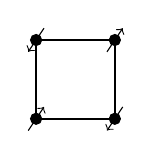
\begin{tikzpicture}[scale=1, every node/.style={font=\small}]
  % Lattice sites
  \foreach \x in {0,1} {
    \foreach \y in {0,1} {
      \filldraw (\x,\y) circle (2pt);
    }
  }

  % Bonds (Heisenberg exchange interactions)
  \draw[thick] (0,0) -- (1,0);
  \draw[thick] (0,1) -- (1,1);
  \draw[thick] (0,0) -- (0,1);
  \draw[thick] (1,0) -- (1,1);

  % Spin arrows
%   \foreach \x in {0,1} {
%     \foreach \y in {0,1} {
%         \draw[->] (\x-.1,\y-.15) -- +(.2,.3);
%     }
%   }
    \draw[->] (-.1,-.15) -- +(.2,.3);
    \draw[<-] (.9,-.15) -- +(.2,.3);
    \draw[<-] (-.1,0.85) -- +(.2,.3);
    \draw[->] (.9,.85) -- +(.2,.3);
\end{tikzpicture}
\end{document}
